\documentclass{letask}

\begin{document}
\begin{titlepage}
\center % Center everything on the page
 
%----------------------------------------------------------------------------------------
%	HEADING SECTIONS
%----------------------------------------------------------------------------------------

\textsc{\LARGE Московский\\[-0.2cm]Физико-Технический Институт\\[0.1cm]\large (государственный университет)}\\[1.5cm] % Name of your university/college
\textsc{\Large Кафедра общей физики}\\[0.1cm] % Major heading such as course name
\textsc{\large Лабораторная работа \textnumero  4.4.1}\\[0.5cm] % Minor heading such as course title

%----------------------------------------------------------------------------------------
%	TITLE SECTION
%----------------------------------------------------------------------------------------

\HRule
\\[0.4cm]
{ \huge \bfseries Амплитудная\\[0.2cm]
дифракционная решетка}
\\[0.6cm] % Title of your document
\HRule
\\[1.5cm]


 
%----------------------------------------------------------------------------------------
%	AUTHOR SECTION
%----------------------------------------------------------------------------------------

\begin{minipage}{0.4\textwidth}
	\begin{flushleft} \large
		\textsf{Студент}
		
		Ришат \textsc{Исхаков} \\[-0.15cm]
		513 группа
	\end{flushleft}
\end{minipage}
~
\begin{minipage}{0.4\textwidth}
	\begin{flushright} \large
		\textsf{Преподаватель}
		
		Александр Александрович \\[-0.15cm]
		\textsc{Казимиров} % Supervisor's Name
	\end{flushright}
\end{minipage}

\begin{bottompar}
	\begin{center}
		
\includegraphics[width = 80 mm]{logo.jpg}
	\end{center}
	{\large \today}

\end{bottompar}
\vfill % Fill the rest of the page with whitespace

\end{titlepage}

\textbf{Цель работы:} исследовать зависимость видности интерференционной картины от разности хода интерферирующих лучей и от их поляризации.

\textbf{В работе используются:} гелий-неоновый лазер, интерферометр Майкельсона с подвижным зеркалом, фотодиод с усилителем, осциллограф С1-76, поляроид, линейка.

\section{Теоретическая часть}

Лазер состоит из двух зеркал, составляющих лазерный резонатор, и расположенной между ними газообразной усиливающей среды, состоящей из гелия и неона. Характерное расстояние между зеркалами ~--~$0.2 \div 1 \m$. 

Излучение распространяется по резонатору в прямом и обратном направлениях. При этом максимальным усилением обладают волны, для которых набег фазы при полном обходе резонатора кратен $2 \pi$. Тогда можно сформулировать условие на разность частот излучения. Так как:
\[ \dfrac{2 \pi}{\lambda}2L = 2 \pi m,	\quad L=m\lambda, \quad \nu_{m}=\dfrac{mc}{2L}, \]
тогда:

\begin{equation}
\label{eq:cond}
\Delta \nu_{m}=\nu_{m+1}-\nu_{m}=\dfrac{c}{2L},
\end{equation}

где $L$ -- длина резонатора, $m$ -- целое число. Поэтому лазер генерирует отдельные типы колебаний, называемые модами, удовлетворяющие условию (\ref{eq:cond}). 

Спектральная ширина отдельной моды определяется добротностью резонатора лазера и мощностью излучения. В He-Ne лазере из-за малого усиления активной среды используются зеркала с высоким отражением. добротность резонатора большая и спектральная ширина моды может быть очень узкой, вплоть до единиц $\Hz$. Ввиду наличия тепловых флуктуаций длины резонатора типичная ширина моды составляет $10^5 \; \Hz$. Количество генерируемых мод определяется шириной спектра усиления активной среды. Эта ширина складывается из естественной ширины линии излучения атомов неона и доплеровского уширения, вызванного тепловым движением атомов. При температуре $400 \K$ ширина по полувысоте спектра излучения газообразного неона равна $1.5 \cdot 10^{9} \; \Hz$.

Вследствие тепловых флуктуаций длина резонатора меняется, в результате чего моды "переползают" с одного края контура на другой, там исчезают, а на другом краю рождаются новые. Таким образом температура нестабильность приводит к медленным изменениям амплитуд колебаний в лазерных модах и числа самих мод.

\begin{wrapfigure}[15]{L}{0.4 \lw}
	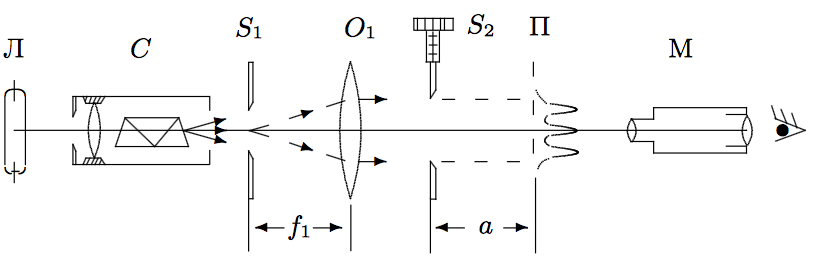
\includegraphics[width =  \lw]{img1}
	\caption{Осциллограмма сигналов фотодиода}
	\label{fig:somelabel}
\end{wrapfigure}

\textbf{Видность интерференционной картины.} Если в плоскости наблюдения две плоские волны с длиной волны $\lambda_{0}$ сходятся под малым углом $\alpha$, то наблюдается интерференционная картина в виде последовательности темных и светлых полос c расстоянием между ними:
\begin{equation}
\label{eq:deltax}
\Delta x = \dfrac{\lambda_{0}}{\alpha}
\end{equation}

Для оценки чёткости интерференционной картины в окрестности некоторой точки используют параметр видимости:
\begin{equation}
\label{eq:seen}
V=\dfrac{I_{max}-I_{min}}{I_{max}+I_{min}},
\end{equation}

где $I_{max}$ и $I_{min}$ -- максимальная и минимальная интенсивности света интерференционной картины вблизи выбранной точки. Человеческий глаз может уверенно различать чередование светлых и темных полос при $V \geq 0,1$. 

Пусть интерферируют две волны с амплитудами $A_{m}$ и $B_{m}$. Если в точке наблюдения разность фаз между волнами равна $k_{m} l$, где $k_{m}$ -- волновое число, $l$ -- разность хода, то интенсивность света в этой точке:
\begin{equation}
\label{eq:intensity}
I_{m} = {A_{m}}^2+{B_{m}}^2+2 A_{m} B_{m} cos(k_{m}l)
\end{equation} 
В максимуме интенсивность $I_{max} = (A_{m}+B_{m})^2$, в минимуме $I_{min} = (A_{m}-B_{m})^2.$ Отсюда видность:
\begin{equation}
\label{eq:seen1}
V_{1} = \dfrac{2 \sqrt{\delta}}{1+\delta},
\end{equation}
где $\delta = (B_{m}/A_{m})^2$.

Рассмотрим влияние спекрального состава на видность интерференционной картины:
\begin{equation}
V_{2}(l) = \dfrac{\sum_{n=1}^{\infty} {A_{n}}^2 cos(\dfrac{2 \pi \Delta \nu n l}{c})}{\sum_{n=1}^{\infty}{A_{n}}^2}.
\end{equation}

Введем также поправку к видности, связанную с углом между плоскостями поляризации падающих волн:
\begin{equation}
V_{3} = cos \beta,
\end{equation}
где $\beta$ -- угол между плоскостями поляризации.
Кроме того, по данным осциллограммы (рис.1) можно определить
\begin{equation}
\delta = \dfrac{h_{1}}{h_{2}}
\end{equation}

\begin{equation}
V = \dfrac{h_{4}-h_{3}}{h_{4}+h_{3}},
\end{equation}

где $V$ -- полная видимость. Если имеют место все три фактора уменьшения видимости: неравенство амплитуд, несовпадение поляризаций и разная оптическая задержка между интерферирующими пучками, то:
\begin{equation}
V = V_{1} \cdot V_{2} \cdot V_{3}.
\end{equation}	
	
\section{Экспериментальная установка}

\begin{figure}[H]
\centering
	\begin{center}
		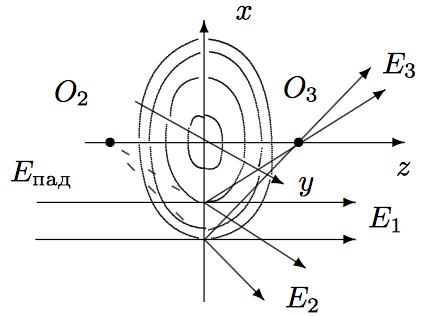
\includegraphics[width = 0.9 \lw]{img2}
	\end{center}
	\caption{Схема экспериментальной установки}
\end{figure}

Экспериментальная установка представляет собой интерферометр Майкельсона, смонтированный на вертикально стоящей плите. Источником света служит гелий-неоновый лазер ($\lambda_{0} = 632,8 \nm$). Пучок лазерного излучения отражается от зеркала З и проходит через ромб Френеля(РФ).

Пучок 1 проходит поляроид $\text{П}_{1}$, отражается под небольшим углом от зеркала $\text{З}_1$, снова проходит поляроид $\text{П}_{1}$ и, частично отражаясь от диагональной плоскости делительного кубика, выходит из интерферометра, попадая на зеркало $\text{З}_3$ и фотодиод ФД. При этом можно вращать $\text{П}_{1}$, изменяя плоскость поляризации.

Пучок 2 проходит линзу Л, поляроид $\text{П}_2$, отражается от зеркала $\text{З}_2$, снова проходит $\text{П}_{2}$, линзу Л и делительный кубик, выходит из интерферометра, попадает на зеркало $\text{З}_3$ и далее на фотодиод ФД. Таким образом, от зеркала $\text{З}_3$ под небольшим углом друг к другу идут на фотодиод два пучка, проходящие через разные плечи интерферометра. Для питания усилителя сигнала фотодиода и управления пьезокерамикой используется блок питания БП.


\section{Установка и параметры измерения}

Расстояние между зеркалами лазера: $65~\cm$.

\subsection*{Зависимость видности от угла $\beta$ поворота поляроида}


\begin{table}[H]
\centering
\caption{Измерим зависимость видности $\nu_3$ от угла поворота поляроида при нулевой разности хода}
\begin{tabular}{|c|c|c|c|c|c|c|c|c|c|c|}
\hline
$\beta, ~^\circ$ & $h_1$ & $h_2$ & $h_3$ & $h_4$ & $\delta$ & $\nu$ & $\nu_1$ & $\nu_3$ & $\cos \beta$ & ${\cos}^2 \beta$ \\ \hline
90      & 0.2   & 1.4   & 1.1   & 2.2   & 0.14     & 0.33  & 0.66    & 0.50    & 0.00         & 0.00           \\ \hline
85      & 0.2   & 1.5   & 1.1   & 2.3   & 0.13     & 0.35  & 0.64    & 0.55    & 0.09         & 0.01           \\ \hline
80      & 0.3   & 1.5   & 1.1   & 2.5   & 0.20     & 0.39  & 0.75    & 0.52    & 0.17         & 0.03           \\ \hline
75      & 0.3   & 1.5   & 1     & 2.6   & 0.20     & 0.44  & 0.75    & 0.60    & 0.26         & 0.07           \\ \hline
70      & 0.4   & 1.4   & 0.9   & 2.8   & 0.29     & 0.51  & 0.83    & 0.62    & 0.34         & 0.12           \\ \hline
65      & 0.4   & 1.4   & 0.8   & 2.8   & 0.29     & 0.56  & 0.83    & 0.67    & 0.42         & 0.18           \\ \hline
60      & 0.5   & 1.4   & 0.7   & 3     & 0.36     & 0.62  & 0.88    & 0.71    & 0.50         & 0.25           \\ \hline
55      & 0.5   & 1.4   & 0.7   & 2.9   & 0.36     & 0.61  & 0.88    & 0.69    & 0.57         & 0.33           \\ \hline
50      & 0.8   & 1.4   & 0.6   & 3.7   & 0.57     & 0.72  & 0.96    & 0.75    & 0.64         & 0.41           \\ \hline
45      & 0.9   & 1.3   & 0.6   & 4     & 0.69     & 0.74  & 0.98    & 0.75    & 0.71         & 0.50           \\ \hline
40      & 1     & 1.3   & 0.5   & 4.2   & 0.77     & 0.79  & 0.99    & 0.79    & 0.77         & 0.59           \\ \hline
35      & 1.2   & 1.3   & 0.5   & 4.6   & 0.92     & 0.80  & 1.00    & 0.80    & 0.82         & 0.67           \\ \hline
30      & 1.3   & 1.4   & 0.5   & 4.6   & 0.93     & 0.80  & 1.00    & 0.80    & 0.87         & 0.75           \\ \hline
25      & 1.3   & 1.4   & 0.5   & 4.8   & 0.93     & 0.81  & 1.00    & 0.81    & 0.91         & 0.82           \\ \hline
20      & 1.4   & 1.4   & 0.5   & 4.8   & 1.00     & 0.81  & 1.00    & 0.81    & 0.94         & 0.88           \\ \hline
15      & 1.5   & 1.3   & 0.5   & 4.9   & 1.15     & 0.81  & 1.00    & 0.82    & 0.97         & 0.93           \\ \hline
10      & 1.5   & 1.3   & 0.5   & 5.1   & 1.15     & 0.82  & 1.00    & 0.82    & 0.98         & 0.97           \\ \hline
5       & 1.6   & 1.4   & 0.5   & 5.3   & 1.14     & 0.83  & 1.00    & 0.83    & 1.00         & 0.99           \\ \hline
0       & 1.7   & 1.4   & 0.4   & 5.4   & 1.21     & 0.86  & 1.00    & 0.87    & 1.00         & 1.00           \\ \hline
\end{tabular}
\end{table}

\begin{figure}[H]
\centering
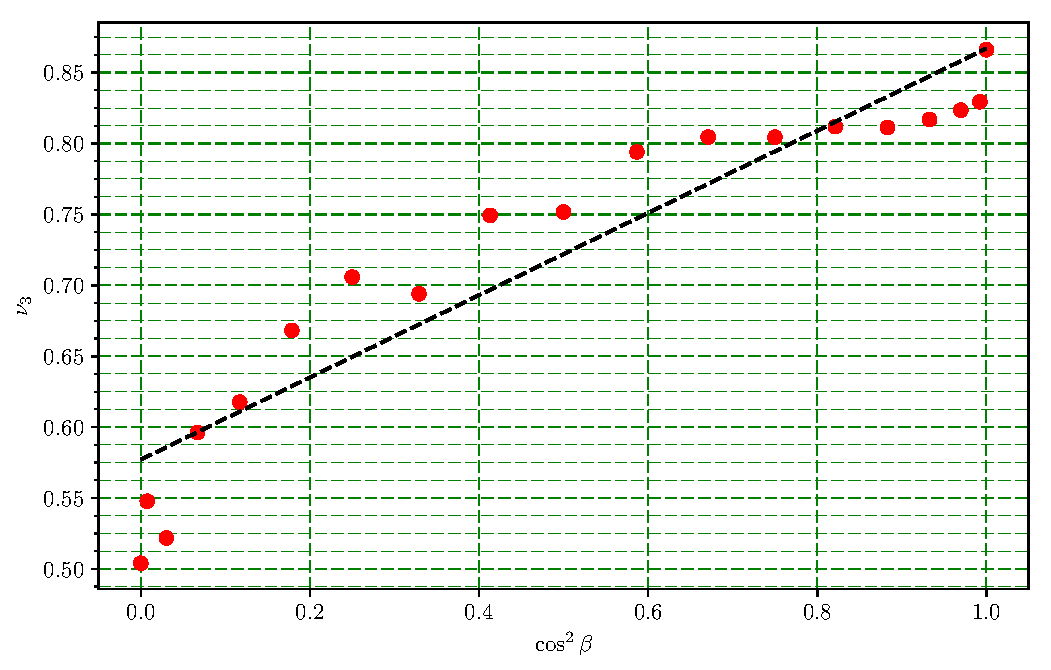
\includegraphics[width = 0.75 \lw]{graph}
\caption{График зависимости $ \nu({\cos}^2 \beta) $}
\end{figure}


\subsection*{Зависимость видности $\nu_2$ от координаты $x$ блока}

\begin{table}[H]
\centering
\caption{Измерим зависимость видности $\nu_2$ от координаты $x$ блока}
\begin{tabular}{|c|c|c|c|c|c|c|c|c|}
\hline
$x$ & $h_1$ & $h_2$ & $h_3$ & $h_4$ & $\delta$ & $\nu$ & $\nu_1$ & $\nu_2$ \\ \hline
10  & 1.2   & 0.7   & 1     & 2.8   & 0.58     & 0.47  & 0.96    & 0.49    \\ \hline
12  & 1.2   & 0.8   & 0.9   & 3.3   & 0.67     & 0.57  & 0.98    & 0.58    \\ \hline
14  & 1.2   & 1.1   & 0.9   & 3.8   & 0.92     & 0.62  & 1.00    & 0.62    \\ \hline
16  & 1.2   & 1.3   & 0.9   & 4.1   & 1.08     & 0.64  & 1.00    & 0.64    \\ \hline
18  & 1.2   & 1.4   & 1     & 4.3   & 1.17     & 0.62  & 1.00    & 0.62    \\ \hline
20  & 1.2   & 1.8   & 1.3   & 4.7   & 1.50     & 0.57  & 0.98    & 0.58    \\ \hline
22  & 1.2   & 1.5   & 1.3   & 4.1   & 1.25     & 0.52  & 0.99    & 0.52    \\ \hline
24  & 1.2   & 0.8   & 1.2   & 2.9   & 0.67     & 0.41  & 0.98    & 0.42    \\ \hline
26  & 1.2   & 0.6   & 1     & 2     & 0.50     & 0.33  & 0.94    & 0.35    \\ \hline
32  & 1.2   & 1.6   & 2.6   & 2.8   & 1.33     & 0.04  & 0.99    & 0.04    \\ \hline
38  & 1.2   & 1.2   & 2.3   & 2.6   & 1.00     & 0.06  & 1.00    & 0.06    \\ \hline
44  & 1.2   & 0     & 1.2   & 1.4   & 0.00     & 0.08  & 1.00    & 0.08    \\ \hline
50  & 0.9   & 1.8   & 2.4   & 2.9   & 2.00     & 0.09  & 0.94    & 0.10    \\ \hline
54  & 0.9   & 1.8   & 2.4   & 2.9   & 2.00     & 0.09  & 0.94    & 0.10    \\ \hline
66  & 1.4   & 3.4   & 4.4   & 4.8   & 2.43     & 0.04  & 0.91    & 0.05    \\ \hline
70  & 1.2   & 2.6   & 3.3   & 4.2   & 2.17     & 0.12  & 0.93    & 0.13    \\ \hline
72  & 1.2   & 3     & 3.2   & 6     & 2.50     & 0.30  & 0.90    & 0.34    \\ \hline
74  & 1.2   & 3     & 3.1   & 7     & 2.50     & 0.39  & 0.90    & 0.43    \\ \hline
76  & 1.2   & 3     & 2.9   & 6.4   & 2.50     & 0.38  & 0.90    & 0.42    \\ \hline
78  & 1.3   & 3.3   & 2.7   & 6     & 2.54     & 0.38  & 0.90    & 0.42    \\ \hline
81  & 1.2   & 3.5   & 2.5   & 5.7   & 2.92     & 0.39  & 0.87    & 0.45    \\ \hline
84  & 1.2   & 3.7   & 2.2   & 5     & 3.08     & 0.39  & 0.86    & 0.45    \\ \hline
\end{tabular}
\end{table}

\begin{figure}[H]
\centering
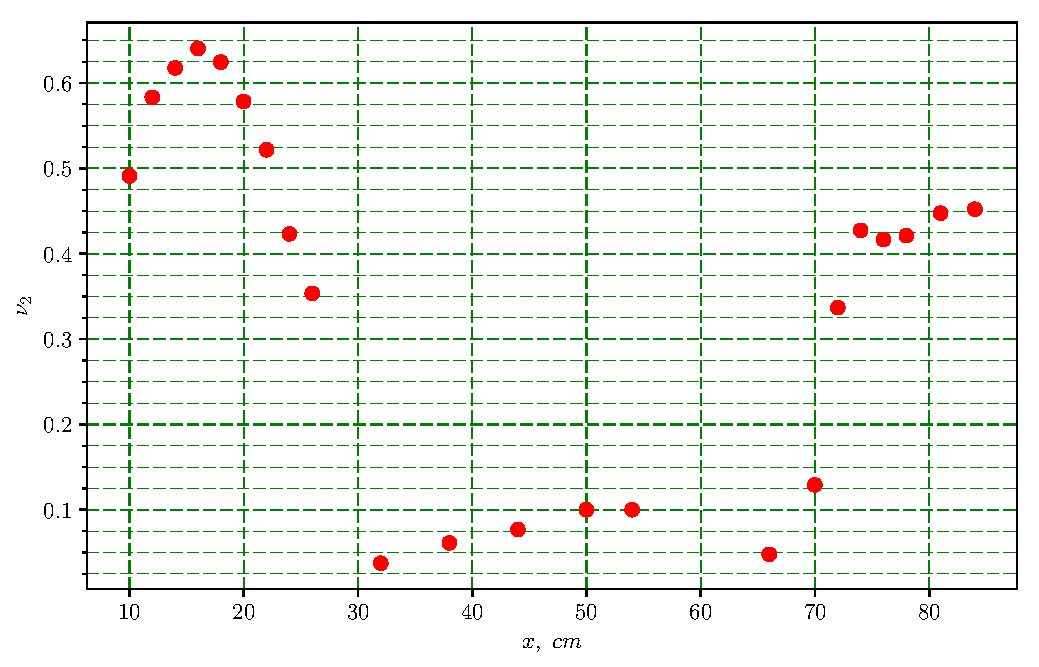
\includegraphics[width = 0.7 \lw]{graph2}
\caption{График зависимости $ \nu_2(x)$}
\end{figure}

По полученному графику определим примерный размер резонатора лазера:
\[ L \approx 77 - 15 = 62~\cm \]

Тогда межмодовое расстояние равно:
\[ \Delta \nu_m = \dfrac{c}{2L} = 2.4 \cdot 10^8~\Hz \]

Полуширина первого максимума: 
\[ l_{1/2} = 16~\cm \]

Тогда диапазон частот, в котором происходит генерация продольных мод оценивается выражением:
\[\Delta F = \dfrac{\sqrt{\ln 2} c}{l_{1/2}} = 13 \cdot 10^8~\Hz \]

Оценим число генерируемых лазером продольных мод:
\[ n \approx 1 + 1.2\dfrac{L}{l_{1/2}} = 6 \]

\section{Вывод}
Исследуя видность интерференционной картины излучения гелий-неонового лазера мы измерили диапазон частот, в котором происходит генерация продольных мод, число продольных мод. Почти точно определили размер резонатора. Зависимость $\nu_2({\cos}^2 \beta$ оказалось линейной, но не проходит через ноль из-за неточности установки и измерений (поляроид не перекрывал свет полностью).
\end{document}
